\documentclass{ximera}

\title{Vectorieel Product}
%\author{Daan Lipkens} %wiskunde on

\begin{document}
\begin{abstract}
\end{abstract}
\maketitle


Het \textbf{vectorieel product} (of kruisproduct) levert een \textbf{vector} als resultaat op, waarvan de grootte exact gelijk is aan de oppervlakte van het parallellogram dat wordt opgespannen door de twee vectoren. 

De richting van het vectorproduct staat steeds \textbf{loodrecht} op het vlak dat gevormd wordt door de twee gegeven vectoren, en de zin is te bepalen met de zogenaamde \textbf{rechterhandregel}.

Het vectorieel product wordt genoteerd met een kruisje:
\[ \vec{c} = \vec{a} \times \vec{b} \]
De grootte van deze nieuwe vector is:
\[ \|\vec{c}\| = \| \vec{a}_y \| \cdot \|\vec{b}\| = \|\vec{a}\| \cdot \sin(\alpha) \cdot \|\vec{b}\| = \| \vec{a}\| \cdot \| \vec{b}\| \cdot \sin(\alpha) \]

%---------------------------
% AFBEELDING: Vectorieel product
\begin{figure}[ht!]
    \captionsetup{width=0.85\textwidth}
    \begin{center}
        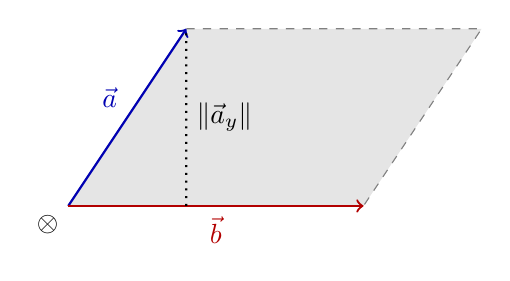
\begin{tikzpicture}[scale=1.5]
            \coordinate (O) at (0,0);
            \coordinate (A) at (1,1.5);
            \coordinate (B) at (2.5,0);
            \coordinate (C) at (3.5,1.5); % A+B
            
            \fill[gray!20] (O) -- (A) -- (C) -- (B) -- cycle;
            
            \draw[->, thick, blue!70!black] (O) -- (A) node[midway, above left]{$\vec{a}$};
            \draw[->, thick, red!70!black] (O) -- (B) node[midway, below]{$\vec{b}$};
            
            \draw[dashed, gray] (A) -- (C) -- (B);
            \draw[dotted, thick, black] (1,0) -- (A) node[midway, right]{$\|\vec{a}_y\|$};
            
            \fill (O) node[below left]{$\otimes$};
        \end{tikzpicture}
    \end{center}
    \caption{De grootte van het vectorieel product $\vec{a} \times \vec{b}$ is gelijk aan de oppervlakte van het parallellogram.}
    \label{fig:vectorieel_product}
\end{figure}
%---------------------------

\begin{remark}[expandable=true,title={Notatie voor de derde dimensie}]\nl
    Een vector waarvan de richting en zin zich \textbf{in het blad} boort (zoals de pijl van een dart die van je wegvliegt) wordt genoteerd met een kruisje: $\otimes$. \\
    Een vector met zin \textbf{uit het blad} (zoals de punt van een dart die naar je toe komt) wordt genoteerd met een puntje: $\odot$.
\end{remark}

\begin{figure}[ht!]
    \captionsetup{width=0.85\textwidth}
    \begin{center}
        
\includegraphics[width=0.4\textwidth]{pic5/appendix/rechterhandregel.png}
    \end{center}
    \caption{De rechterhandregel bepaalt de zin van het vectorieel product.}
    \label{fig:rechterhandregel}
\end{figure}

\end{document}